% Options for packages loaded elsewhere
\PassOptionsToPackage{unicode}{hyperref}
\PassOptionsToPackage{hyphens}{url}
%
\documentclass[
]{article}
\usepackage{amsmath,amssymb}
\usepackage{iftex}
\ifPDFTeX
  \usepackage[T1]{fontenc}
  \usepackage[utf8]{inputenc}
  \usepackage{textcomp} % provide euro and other symbols
\else % if luatex or xetex
  \usepackage{unicode-math} % this also loads fontspec
  \defaultfontfeatures{Scale=MatchLowercase}
  \defaultfontfeatures[\rmfamily]{Ligatures=TeX,Scale=1}
\fi
\usepackage{lmodern}
\ifPDFTeX\else
  % xetex/luatex font selection
\fi
% Use upquote if available, for straight quotes in verbatim environments
\IfFileExists{upquote.sty}{\usepackage{upquote}}{}
\IfFileExists{microtype.sty}{% use microtype if available
  \usepackage[]{microtype}
  \UseMicrotypeSet[protrusion]{basicmath} % disable protrusion for tt fonts
}{}
\makeatletter
\@ifundefined{KOMAClassName}{% if non-KOMA class
  \IfFileExists{parskip.sty}{%
    \usepackage{parskip}
  }{% else
    \setlength{\parindent}{0pt}
    \setlength{\parskip}{6pt plus 2pt minus 1pt}}
}{% if KOMA class
  \KOMAoptions{parskip=half}}
\makeatother
\usepackage{xcolor}
\usepackage[margin=1in]{geometry}
\usepackage{graphicx}
\makeatletter
\def\maxwidth{\ifdim\Gin@nat@width>\linewidth\linewidth\else\Gin@nat@width\fi}
\def\maxheight{\ifdim\Gin@nat@height>\textheight\textheight\else\Gin@nat@height\fi}
\makeatother
% Scale images if necessary, so that they will not overflow the page
% margins by default, and it is still possible to overwrite the defaults
% using explicit options in \includegraphics[width, height, ...]{}
\setkeys{Gin}{width=\maxwidth,height=\maxheight,keepaspectratio}
% Set default figure placement to htbp
\makeatletter
\def\fps@figure{htbp}
\makeatother
\setlength{\emergencystretch}{3em} % prevent overfull lines
\providecommand{\tightlist}{%
  \setlength{\itemsep}{0pt}\setlength{\parskip}{0pt}}
\setcounter{secnumdepth}{5}
\usepackage[T1]{fontenc}
\usepackage[utf8]{inputenc}
\usepackage[spanish, provide=*]{babel}
\usepackage{floatrow}
\floatsetup[figure]{capposition=top}
\usepackage{array}
\usepackage{fancyhdr}
\usepackage{graphicx}
\usepackage{hyperref}
\usepackage{pdfpages}
\usepackage[defaultfam,tabular,lining]{montserrat}
\usepackage{xcolor}
\usepackage[font=bf]{caption}
\definecolor{colortitles}{HTML}{145765}
\definecolor{colorborder}{HTML}{337E8C}
\usepackage{colortbl}
\arrayrulecolor{colorborder}
\usepackage{caption}
\captionsetup[table]{position=above,name=Tabla}

\ifLuaTeX
  \usepackage{selnolig}  % disable illegal ligatures
\fi
\usepackage{bookmark}
\IfFileExists{xurl.sty}{\usepackage{xurl}}{} % add URL line breaks if available
\urlstyle{same}
\hypersetup{
  hidelinks,
  pdfcreator={LaTeX via pandoc}}

\author{}
\date{\vspace{-2.5em}2025-02-17}

\begin{document}

\fontsize{11.5}{13}
\fontseries{c}
\selectfont

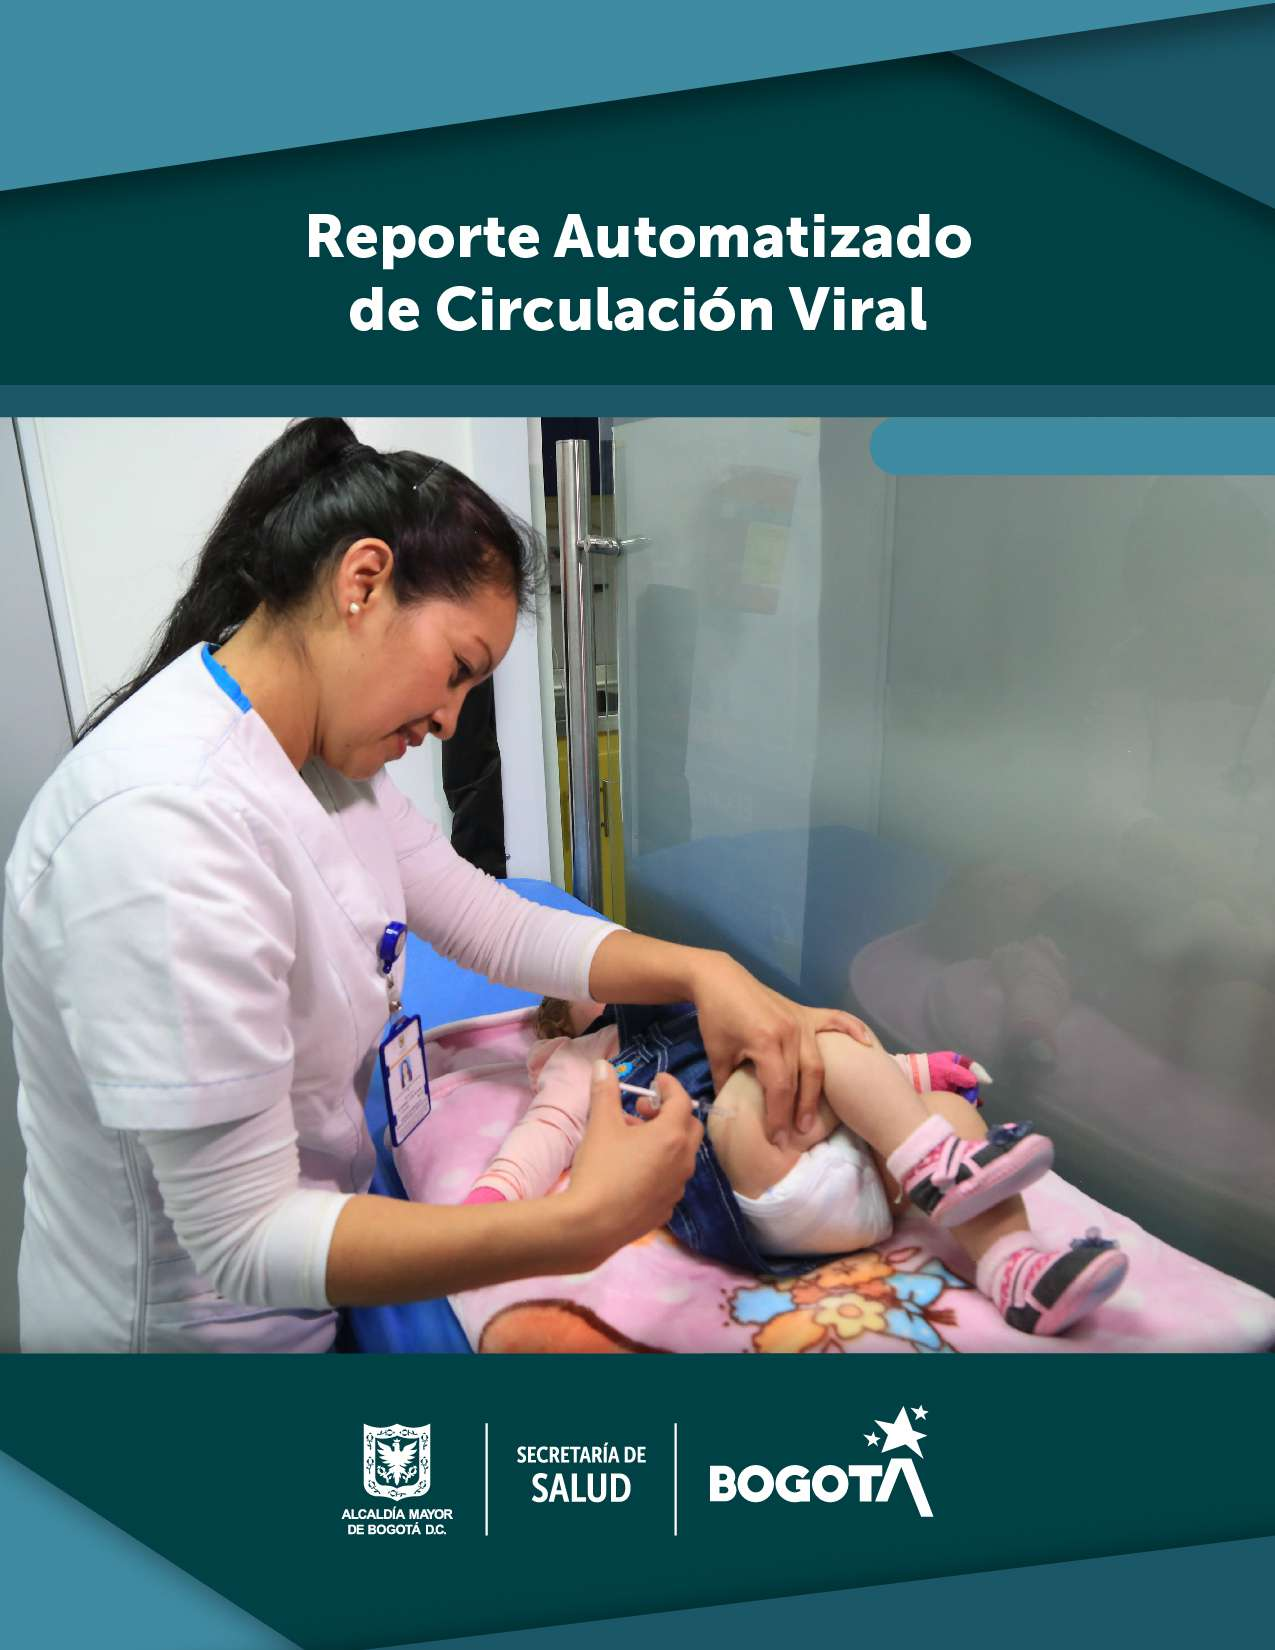
\includepdf[pages={1}]{cover.pdf}

\begin{center}
{\color{colortitles} Alcalde Mayor de Bogotá\\}
Carlos Fernando Galán Pachón\\~\\


{\color{colortitles} Secretario Distrital de Salud\\}
Gerson Orlando Bermont Galavis\\~\\


{\color{colortitles} Subsecretario de Salud Pública\\}
Manuel Alfredo González Mayorga\\[0.4in]


{\color{colortitles} Coordinación general del documento\\~\\}


{\color{colortitles} Directora de Epidemiología, Análisis y Gestión de\\ 
Políticas de Salud Colectiva\\}
Diane Moyano Romero\\~\\


{\color{colortitles} Subdirectora de Vigilancia en Salud Pública\\}
Sol Yiber Beltran Aguilera\\[0.5in]


{\color{colortitles} Autor\\~\\}
{\color{colortitles} Laboratorio de Salud Pública\\}
Sandra Liliana Gómez Bautista\\
Paula Andrea Borda Osuna\\[0.6in]


{\color{colortitles} Coordinación Editorial\\~\\}

{\color{colortitles} Oficina Asesora de Comunicaciones en Salud\\}
María Juliana Silva Amado\\~\\


{\color{colortitles} Corrección de estilo\\}
José Aldemar Garzón González\\~\\


{\color{colortitles} Diseño y diagramación\\}
Harol Giovanny León Niampira\\~\\


{\color{colortitles} Fotografía portada\\}
www.saludcapital.gov.co\\~\\


{\color{colortitles}
Secretaría Distrital de Salud\\
Carrera 32 No. 12-81\\
Conmutador: 364 9090\\
Bogotá, D. C. - 2024\\
www.saludcapital.gov.co\\}
\end{center}

\pagenumbering{gobble}
\pagenumbering{arabic}

\newpage

\begin{flushleft}
{\color{colortitles} \section{Virus respiratorios}}
\end{flushleft}

Durante 2025, el Laboratorio de Salud Pública (LSP) continúa apoyando la
vigilancia de la infección respiratoria aguda en Bogotá, mediante el
procesamiento de muestras remitidas por instituciones centinela de los
eventos: Enfermedad Similar a Influenza (ESI) que son pacientes
ambulatorios, de pacientes hospitalizados por Infección Respiratoria
Aguda Grave (IRAG) y de IRAG inusitado que se presente en cualquier
institución de la ciudad.

Las muestras previamente son procesadas por RT-PCR para SARS-CoV-2 y
después continúan su análisis con: panel respiratorio Allplex y reacción
en cadena de la polimerasa con transcriptasa inversa (RT-PCR) para el
diagnóstico de los principales agentes a los que se les atribuye el
IRAG.

\begin{verbatim}
## On branch main
## Your branch is up to date with 'origin/main'.
## 
## nothing to commit, working tree clean
\end{verbatim}

ESTOS SON LOS DATOS A ALMACENAR:

\begin{verbatim}
## [1] TRUE
\end{verbatim}

\begin{verbatim}
## [1] "Iniciando el almacenamiento de los archivos en formato RDS..."
\end{verbatim}

\begin{verbatim}
## [1] "Archivos RDS guardados exitosamente en 'inst/extdata/library-labrep/'."
## [1] "Enviando los cambios a GitHub..."
\end{verbatim}

\begin{verbatim}
## [1] "cambios subidos exitosamente a GitHub."
\end{verbatim}

\begin{verbatim}
## On branch main
## Your branch is up to date with 'origin/main'.
## 
## nothing to commit, working tree clean
\end{verbatim}


\includepdf[pages={1}]{back_cover.pdf}

\end{document}
